\chapter{Solving the Shortest Path Problem}
\label{chapter:solvingspp}

In this chapter we discuss the algorithms
that solve the shortest path problem that are
applicable for the transportation network.
\marginpar{TODO\\Big O\\Analysis}

\section{Generic Shortest Path Algorithm (GSP)}

A family of algorithms exist for solving SPP,
in this section we describe the generic case for these
algorithms.

All of these algorithms depend on solving 
a label vector ($d_1, d_2,\dots d_v$) \citep{Klunder}.
Each $d_v$ keeps the least distance of of any path going from $s$ to $v$, $d_v = \infty$ if no paths has been found.
A shortest path is optimal when it satisfies the following conditions:
\begin{align}
    d_v \leq d_u + c_{uv}, \quad \forall(u,v) \in \mathcal{A}, \label{eq:Bellman1}\\
    d_v  =   d_u + c_{uv}, \quad \forall(u,v) \in \mathcal{P}.
\end{align}
The inequalities~(\ref{eq:Bellman1}) is called the Bellman's conditions \citep{Bellman}.
\marginpar{Bellman's \\conditions}
In other words,
we wish to find a label vector $d$ which satisfy the Bellman's conditions for all of the vertices in the graph.
To maintain the label vector, the algorithm uses a candidate list $\mathcal{Q}$ to store the label distances.

In the label vector,
a node is said to be unvisited when $d_u = \infty$,
scanned when $d_u \neq \infty$ and is still in the candidate list,
and labelled when the node has been retrieved from the candidate list and its distance label cannot be updated further.

In the generic shortest path algorithm,
we start by putting the origin node in the queue,
and then iteratively find the arc that violates the Bellman's condition (i.e., $d_v > d_u + c_{uv}$),
distance labels are set to a value which satisfy condition (\ref{eq:Bellman1}) to the corresponding node of that arc.
Shortest path going from $s$ to all other nodes in $\mathcal{V}$ is found when (\ref{eq:Bellman1}) is satisfied for all arcs in $\mathcal{A}$.
It may not be obvious but negative costs are permitted in the GSP but not negative cost cycles.

We use $p_u$ to denote the predecessor of node $u$;
shortest path can be constructed by following the predecessor of destination node $t$ back to origin node $s$.
\marginpar{TODO}

The following pseudo code describes the generic shortest path algorithm mentioned above,
with an extra constraint than a normal GSP: travelling through zone nodes are not allowed.
\begin{algorithm}
    \caption{The Generic Shortest Path Algorithm \citep{Klunder}}
    \begin{algorithmic}[1]
        \Procedure{GenericShortestPath}{$s$}
        \State $\mathcal{Q} \gets \mathcal{Q} \cup \{s\}$ \Comment{Initialisation}
        \State $p_s \gets -1$ \Comment{Origin has no predecessor}
        \State $d_s \gets 0$
        \ForAll {$ u \in \mathcal{V} : u \neq s $} \Comment{All nodes unvisited except the source}
            \State $d_u \gets \infty$
        \EndFor

        \While{ $\mathcal{Q} \neq \emptyset$ }
        \State $ u \gets \text{top}(\mathcal{Q}) $ \Comment{get pivot node}
        \State $ u \gets \mathcal{Q} \setminus \{u\} $
            \If{ $u \neq \text{zone} $}
            \ForAll {$v : (u, v) \in \mathcal{A}$} \Comment{For all outgoing arcs from $u$}
                    \If {$d_u + c_{vw} < d_v$}
                        \State $d_v \gets d_u + c_{vw}$
                        \State $p_v \gets u$
                        \If {$v \notin \mathcal{Q}$} \Comment{Include node $v$ if unvisited}
                        \State $\mathcal{Q} \gets \mathcal{Q} \cup \{v\}$
                        \EndIf
                    \EndIf
                \EndFor
            \EndIf
        \EndWhile
        \EndProcedure
    \end{algorithmic}
\end{algorithm}
\marginpar{TODO\\check correctness}

Note GSP is the generic case for a family of algorithms
that use different implementations of the candidate list $\mathcal{Q}$ \citep{mplomer},
of which solve either the one-source or the point-to-point shortest path problem.

\section{Label Correcting Algorithm}
\label{section:labelcorrectingalgorithm}
The GSP is addressed as a label correcting algorithm when the candidate list is changed to
a first in first out (FIFO) queue.
Given the arc costs can be negative (no negative cycle),
and in order to satisfy the Bellman's conditions for all arcs,
the algorithm has to scan all arcs in $\mathcal{A}$ $V-1$ (number of nodes-1) times,
giving a time complexity of $O(mn)$.

In this algorithm,
the distance labels do not get permanently labelled when a pivot node is retrieved from the queue,
another node may 'correct' this node's distance label again,
thus the name label correcting algorithm.
This algorithm is also called the Bellman–Ford–Moore algorithm credited to Bellman, Ford and Moore \citep{Bellman,Ford, Moore}.


\section{Label Setting Algorithm}
\label{section:labelsettingalgorithm}
The classical algorithm for solving the single-source shortest path problem is the Label Setting Dijkstra's algorithm.
Conceptually the algorithm grows a shortest path tree from the source node radially outward.
The algorithm is said to be label setting as when the pivot node is retrieved from the queue,
the node gets permanently labelled,
the shortest path going to this node is then solved,
the distance label on this pivot node gives the length of the shortest path.
In order to do this, 
the priority queue is modified to always have the minimum distance label in front of the queue.
Hence the algorithm will iterate through all successive pivot nodes exactly once,
labelling pivot nodes in the order of non-decreasing distance labels.



The advantage of this algorithm over the label correcting algorithm is
that all nodes are only visited once,
and the shortest path tree grows outward radially.
Combining these two feature,
it is clear that when the pivot node is the destination node and is 
labelled,
we can stop the algorithm for the point to point SPP case,
which is desirable for the Path Equilibration method.
Modifying Step 1 of the Dijkstra Algorithm gives

\begin{algorithm}
    \caption{Point to Point Label Setting Algorithm (Dijkstra)}
    \begin{algorithmic}[1]
        \Procedure{Dijkstra}{$s, t$}
        \State $\mathcal{Q} \gets \{s\}$ \Comment{Initialisation}
        \State $p_s \gets -1$
        \State $d_s \gets 0$
        \ForAll {$ u \in \mathcal{V} : u \neq s $} \Comment{All nodes unvisited except the source}
            \State $d_u \gets \infty$
        \EndFor

        \While{ $\mathcal{Q} \neq \emptyset$ }
            \State $ u \gets \text{top}(Q) $
            \State $ \mathcal{Q} \gets \mathcal{Q} \char`\\ \{u\} $
            \If{ $u = t$ }
                \State \text{Terminate Procedure}
            \EndIf
            \If{ $u \neq \text{zone} $}
            \ForAll {$v : (u, v) \in \mathcal{A}$} \Comment{For all outgoing arcs from $u$}
                    \If {$d_u + c_{vw} < d_v$}
                        \State $d_v \gets d_u + c_{vw}$
                        \State $p_v \gets u$
                        %\If {$v \notin \mathcal{Q}$} \Comment{Include node $v$ if unvisited}
                        \State $\mathcal{Q} \gets \mathcal{Q} \cup \{v\}$
                        %\EndIf
                    \EndIf
                \EndFor
            \EndIf
        \EndWhile
        \EndProcedure
    \end{algorithmic}
\end{algorithm}
Note a path will not be found if the queue becomes empty,
but this stopping condition is safe because we known a path
always exist between an O-D pair.


\subsection{Heap Implementation}
Various implementations of the Heap data structure exist,
with each implementation have some advantages than the other,
for example faster tree balancing, faster push or pop.

We examine 6 different Heap implementations from the C++ Boost Heap Library \citep{BoostHeap}:
\begin{table}[H]
    \centering
    \begin{tabular}{cccccc}
                        & top() & push()    & pop()     & increase() & decrease() \\
        d-ary (Binary)  & O(1)  & O(log(N)) & O(log(N)) & O(log(N))  & O(log(N))  \\
        d-ary (Ternary) & O(1)  & O(log(N)) & O(log(N)) & O(log(N))  & O(log(N))  \\
        Binomial        & O(1)  & O(log(N)) & O(log(N)) & O(log(N))  & O(log(N))  \\
        Fibonacci       & O(1)  & O(1)      & O(log(N)) & O(1)       & O(log(N))  \\
        Pairing         & O(1)  & O($2^{2*\log(\log(N))}$) & O(log(N)) & O($2^{2*\log(\log(N))}$) & O($2^{2*\log(\log(N))}$) \\
        Skew            & O(1)  & O(log(N)) & O(log(N)) & O(log(N)) & O(log(N))   
    \end{tabular}
    \caption{C++ Boost Heap Implementations with Comparison of Amortized Complexity}
    \label{table:heaps}
\end{table}
Where N is the number of elements in the Heap tree, and all time complexities are measured in amortized time.
(the average run time if the operation is run for a long period of time,
average out worse case and best case).

We are interested in using these Heap data structures rather than the standard STL priority queue is because of one reason:
the decrease (or increase) function.
The decrease (or increase) function is referred as the decrease-key (or increase-key) operation,
which updates the value of the key in the Heap tree.
Decrease-key is used for a min-heap and increase-key for a max-heap tree.
For the Dijkstra's algorithm,
often nodes are scanned multiple times in the label updating step,
instead of adding the node again into the Heap tree,
we can use decrease-key on the node,
updating its distance label.
This means we can reduce the size of the Heap tree and run time by using decrease-key
rather than adding the same node (different distance label) in the queue again.

\begin{comment}
Thus we change Step 2 of the GSP
\begin{verbatim}
Step 2: Label update
    if u is not a zone node then
        for each outgoing arc (u,v) \in \mathcal{A} do
            if d_u + c_{uv} < d_v then
                d_v := du + c_{uv}
                p_v := u
                if v \notin Q then
                    add v to Q
                else
                    decrease-key(v)
                end if
            end for
    end if
\end{verbatim}
\end{comment}

In table~\ref{table:heaps},
we can observe the Fibonacci Heap has a very interesting time complexity,
constant amortized time for the push, pop and increase-key operation time.
But the fact is,
we do not know how much constant time it really uses.
This also applies to all the other operations.
And since we do not know the time constant for all the operations,
and with different sparsity of the networks,
we need to experiment with all of them.

C++ Boost Library Heaps are implemented as max-heaps,
which means in order to use the Fibonacci O(1) increase-key function,
we need to negate the distance labels when we add them into the Heap


All of these run times are slower than the STL version of the Heap.
Upon inspection,
it is found that the increase-key operation is used about between 5\% to 10\%
\marginpar{TODO\\actual\\count}
of the time,
which means the graphs are not dense enough for these Heap structures to outperform a
simple array based priority queue.

\section{Bidirectional Dijkstra}
\section{A* Algorithm}
Up until now,
the Dijkstra's algorithm does not take into account the location of the destination,
the shortest path tree is grown out radially until the destination is labelled.
In a traditional graph where actual distances are used for the distance labels,
heuristic can be used to direct the shortest path tree to grow toward the destination.
\marginpar{TODO\\diagram}
If the heuristic estimate is the distance from each node to the destination,
and the estimate is smaller than or equal to the actual distance going to that destination,
then a shortest path can be found. This is called A*.
Formally we define the following: Let $h_v$ be a heuristic estimate from node $v$ to $t$,
apply Bellman's condition an optimal solution exist, that is 
$ h_v \leq h_u + c_{uv}, \quad \forall(u,v) \in \mathcal{A} $.
In other words, the heuristic estimate for each node need to always under estimate the actual distance
going from the node to the destination.

It is proven using geographical coordinates and euclidean distance as the heuristic estimate,
A* is guaranteed to work with a huge run time speed up by scanning very few nodes.

In our Path Equilibration method,
we can no longer use geographical coordinates and euclidean distance for the heuristic estimate,
this is because we use travel times as the distances for the arcs.
Although distance is included in the calculation,
we cannot guarantee it to under estimate the travel times.

By analysing the travel times function (Figure~\ref{fig:flowfunction}),
we can see that it is a non-decreasing function with the lowest value being the zero flow travel times,
which means if we use the zero flow travel times as the heuristic estimate,
it is assured that it will always under estimate the travel time for that arc,
because no travel time can be lower than the zero flow travel at any time.

\begin{figure}[H]
    \centering
    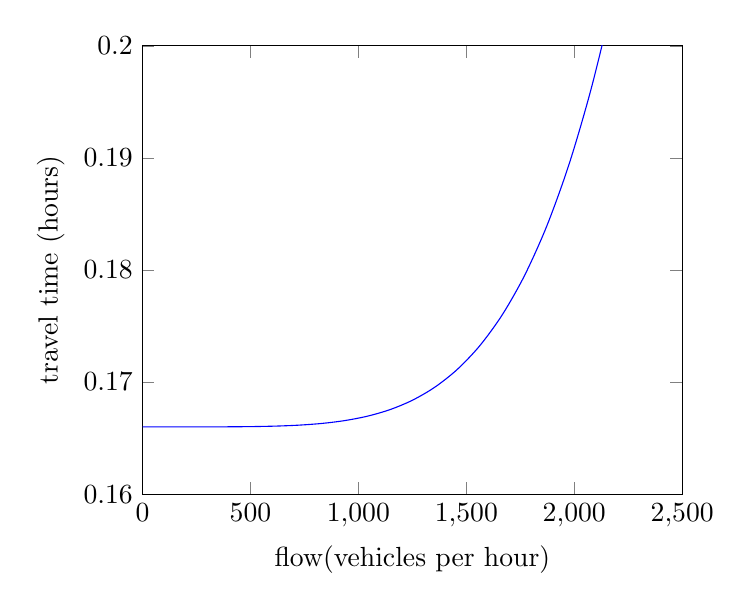
\begin{tikzpicture}
        \begin{axis}
            [
                domain=0:2500,
                black, no markers, smooth,
            %xtick=\empty, ytick=\empty,
                xlabel=flow(vehicles per hour), ylabel=travel time (hours),
                xmin=0,xmax=2500,
                ymin=0.16,ymax=0.2,
                yticklabel style={/pgf/number format/fixed, /pgf/number format/precision=3}
            ]
            \addplot {0.166*(1+0.15*(x/2000)^5)}; 
        \end{axis}
    \end{tikzpicture}
    \caption{Travel time function.}
    \label{fig:flowfunction}
\end{figure}
\marginpar{TODO\\correct\\diagram\\show\\zero flow}

Modifying Step 1 of the GSP for A*:
\begin{algorithm}
    \caption{A* Algorithm}
    \begin{algorithmic}[1]
        \Procedure{AStar}{$s, t$}
        \State $\mathcal{Q} \gets \{s\}$ \Comment{Add node $s$ with $d_s = h_s$}
        \State $p_s \gets -1$
        \State $d_s \gets 0$
        \ForAll {$ u \in \mathcal{V} : u \neq s $} \Comment{All nodes unvisited except the source}
            \State $d_u \gets \infty$
        \EndFor

        \While{ $\mathcal{Q} \neq \emptyset$ }
        \State $ u \gets \text{top}(Q) $ \Comment{Remove $u$ such that $d_u + h_u = \displaystyle\min_{v \in \mathcal{Q}} \{ d_v + h_v \} $}
            \State $ \mathcal{Q} \gets \mathcal{Q} \char`\\ \{u\} $
            \If{ $u = t$ }
                \State \text{Terminate Procedure}
            \EndIf
            \If{ $u \neq \text{zone} $}
            \ForAll {$v : (u, v) \in \mathcal{A}$} \Comment{For all outgoing arcs from $u$}
                    \If {$d_u + c_{vw} < d_v$}
                        \State $d_v \gets d_u + c_{vw}$
                        \State $p_v \gets u$
                        %\If {$v \notin \mathcal{Q}$} \Comment{Include node $v$ if unvisited}
                        \State $\mathcal{Q} \gets \mathcal{Q} \cup \{v\}$ \Comment{Add node $v$ with $d_v = d_u + c_{vw} + h_v$}
                        %\EndIf
                    \EndIf
                \EndFor
            \EndIf
        \EndWhile
        \EndProcedure
    \end{algorithmic}
\end{algorithm}


Comparing the Dijkstra and A* algorithm's result (Table~\ref{table:dijkstraresult} and \ref{table:astarresult}),
we see an approximately 5 times improvement.
By looking at the shortest path tree generated
by the ChicagoSketch network,
there are only a few scanned nodes,
the path goes straight to the destination.
(TODO reference) says the closer the heuristic is to the actual
distance,
the better/faster shortest path calculation,
by looking at the travel time function (Figure~\ref{fig:flowfunction}, we can see the slope
is really shallow near the start,
and by comparing the initial flow and final flow (TODO, data),
\marginpar{TODO}
they are very close so the final flow is very close to the
initial flow,
which means the heuristic is a very good estimation,
which is our A* is very fast.

\section{Bidirectional A*}
\section{Preprocessing}
